% chktex-file 3 chktex-file 9 chktex-file 10 chktex-file 17 chktex-file 18 chktex-file 36
\section*{Exercise 5.}

Consider the function
\[ f(x) = \angles{c,x} - \sum_{j = 1}^m \log(1-\angles{a_j,x}) - \sum_{i = 1}^n \log(1-x_i^2). \]
Take $n = 5000$ and $m = 2000$, and vectors $c,a_j$ chosen arbitrarily such that $\|a_j\| = 1$. For every method initiate the iterations in $x_0 = 0$ and the termination criterion in the form $\|\nabla f(x_k)\| \leq \varepsilon$. Graph $\log(f(x_k)-f^*)$ on each iteration (estimating the best possible $f^*$) and indicate the total time each method takes.

\begin{enumerate}[label=\alph*)]
    \item Use the gradient method with constant step size.
    \item Use the gradient method with backtracking for different parameter values.
    \item Use the gradient method with backtracking and some Goldstein of Wolfe conditions with different parameter values.
    \item Use Newton's method
\end{enumerate}

\textbf{Solution:}

With the objective of hasting the execution of the functions (especially the hessian), I had to vectorize them. We're going to define some elementwise functions for matrices. Some of them are known as the Hadamard products
\[ \odot: \R^{m\times n} \times \R^{m\times n} \to \R^{m\times n},\hspace{1em} (A\odot B)_{ij} = A_{ij}\cdot B_{ij}, \]
\[ \oslash: \R^{m\times n} \times \R^{m\times n} \to \R^{m\times n},\hspace{1em} (A\oslash B)_{ij} = \frac{A_{ij}}{B_{ij}}, \]
\[ \square^{\circ k}: \R^{m\times n} \to \R^{m\times n},\hspace{1em} (A^{\circ k})_{ij} = A_{ij}^k, \]
\[ \log_\circ: \R^{m\times n}_+ \to \R^{m\times n}, \hspace{1em} (\log_\circ(A))_{ij} = [\log(A_{ij})]_{ij}.\]
\[ \diag: \R^{n} \to \R^{n\times n}, \hspace{1em} \diag(x) = \left[ \begin{matrix}
    x_1 & & \\
    & \ddots & \\
    & & x_n
\end{matrix} \right].\]

Now, we can express $f$ in terms of the previous operations,
\[ \hspace*{-4em} f(x) = f_1(x) + f_2(x)+ f_3(x),
\hspace{4em} 
\everymath{\displaystyle}
\arraycolsep=1.8pt\def\arraystretch{1.5}
\begin{array}{rcl}
    f_1(x) & = & c^T x,\\
    f_2(x) & = & - \1_{m}^T\log_\circ(\1_m - A^T x),\\
    f_3(x) & = & - \1_{n}^T\log_\circ(\1_n - x^{\circ 2}).
\end{array} \]
\[ \everymath{\displaystyle}
\arraycolsep=1.8pt\def\arraystretch{1.5}
\begin{array}{rcl}
    Df_1(x) & = & c,\\
    Df_2(x) & = & - A(\1_m - A^T x)^{\circ -1},\\
    Df_3(x) & = & - (2x)\oslash(1-x^{\circ 2}).
\end{array}
\hspace{4em} 
\begin{array}{rcl}
    Hf_1(x) & = & 0_{n\times n},\\
    Hf_2(x) & = & - (A\odot(\1_m - A^T x)^{\circ -2}) A^T,\\
    Hf_3(x) & = & - \diag((2x^{\circ 2} + 2)\oslash(1-x^{\circ 2})^{\circ 2}).
\end{array}
\]

For the previous operations, $A = [a_1 | \cdots | a_m] \in \R^{n\times m}$ is the matrix with vectors $a_j$ on the columns, $\1_m \in \R^m,\; \1_n \in \R^n$ are vectors with ones for entries. It can be shown that all the previous functions coincide with the functions required by the exercise, but it's not in the scope of this solution.

Now, regarding the code, I'm using the same framework I used for exercise 3. The functions are defined as follows,
\begin{minted}{python}
    n = 5000
    m = 2000
    c = np.random.normal(0,1,n)
    a = np.random.normal(0,1,(n,m))
    a = a/norm(a.T, axis = 1) # Uniformly distributed over S^{m-1}

    f = lambda x: c.T@ x - sum(np.log(1-a.T@ x) - sum(np.log(1-x**2)))
    Df = lambda x: c - a@(1/(1-a.T@ x))  - (2*x)/(1-x**2)
    Hf = lambda x: 0 - a*(1/(1-a.T@ x)**2)@ a.T - np.diag(2*(x**2 + 1)/(1-x**2)**2)
\end{minted}

However, I had to make a slight modification to the methods because $f$ is not defined for every $x\in \R^n$. That is because
\[ \dom(f_2) = \left\{ x\in\R^n \;:\; \underbrace{A^T x < \1_m}_{\mbox{\tiny{simplex}}} \right\} \]
\[ \dom(f_3) = \left\{ x\in\R^n \;:\; \underbrace{ \|x\|_\infty^2 = \max(x_i^2) < \1_m}_{\mbox{\tiny{open square}}} \right\}. \]
Furthermore, I believe the the further failure of the implementations presented here are due to the fact that the optimization here is constrained.

\subsection*{Newton's method}

For the Newton's method I used almost the same implementation. But the initial $\alpha_k$ is chosen in such way that $f(x_k + \alpha_k p_k)$ is defined. 
\begin{minted}{python}
    def newton(alpha, gamma, rho, iterations, x_0, f, Df, Hf):
        ...
        i = 0
        while not is_in_domain(x_k_temp) and i < 200:
            alpha_k *= rho
            x_k_temp = x_k+alpha_k*p_k
            i += 1
        print(is_in_domain(x_k_temp))
        
        if not is_in_domain(x_k_temp):
            break
        alpha_k = backtracking(alpha_k, gamma, rho, x_k, f_k, Df_k, p_k)
        ...
\end{minted}

The results were dissapointing though. $\|Df_k\| < \varepsilon$ only happened when $\varepsilon = 4.2$ (I believe due to accumulations in computation errors), but the method converged eventually to some number (which isn't the minimum of the function). The following graphics show the results of Newton's method.

\begin{figure}[H]
    \centering
    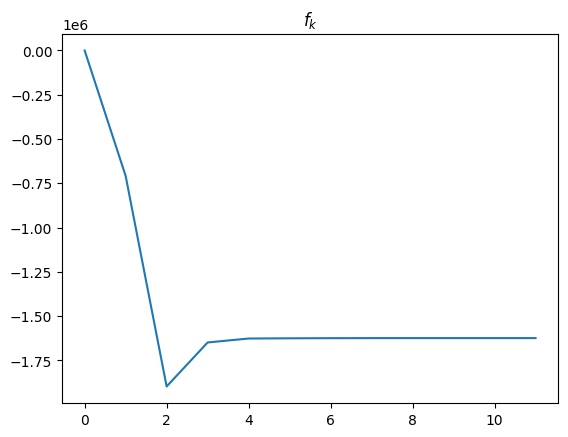
\includegraphics[width=0.45\textwidth]{../pictures/hw2ex5.4.png}
    \hfill
    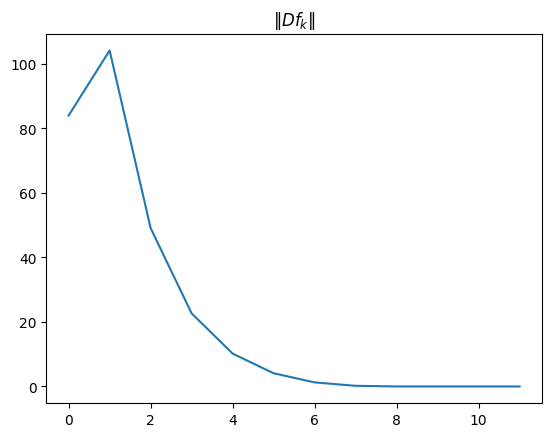
\includegraphics[width=0.45\textwidth]{../pictures/hw2ex5.4.1.png}
\end{figure}

For the other methods the results weren't any better. For constant step size gradient descent, $x_k$ falls of the domain every time with many combinations of parameters. For gradient descent with backtracking $\|Df_k\|$ increases too fast and also falls of the domain. I used all the time I had left trying to analice what went wrong with the implementation so I didn't implement Goldstein or Wolfe conditions.